\documentclass[]{article}

%opening
\title{4F13 Probabilistic Machine Learning - True Skill Ranking}
\author{Candidate: 5562E}

%packages
\usepackage[margin=0.5in]{geometry}
\usepackage[export]{adjustbox}
\usepackage{graphicx}
\usepackage{amsmath}
\usepackage{amssymb}
\usepackage{hyperref}
\usepackage{caption}
\usepackage{subcaption}
\usepackage{parskip}
\usepackage{listings}
\usepackage{pdfpages}
\usepackage{bbm}

%package setup
\graphicspath{{./img/}}
\DeclareMathOperator*{\argmax}{arg\,max}
\DeclareMathOperator*{\argmin}{arg\,min}

%custom commands
\newcommand{\dft}{\mathcal{F}}
\newcommand{\idft}{\mathcal{F}^{-1}}
\newcommand{\Xcal}{\mathcal{X}}
\newcommand{\Ncal}{\mathcal{N}}
\newcommand{\cmplx}{\mathbb{C}}
\newcommand{\Lcal}{\mathcal{L}}
\newcommand{\indep}{\perp \!\!\! \perp}
\newcommand{\figwidth}{0.6\linewidth}

%section numbering
\renewcommand{\thesubsection}{\alph{subsection}}

\begin{document}

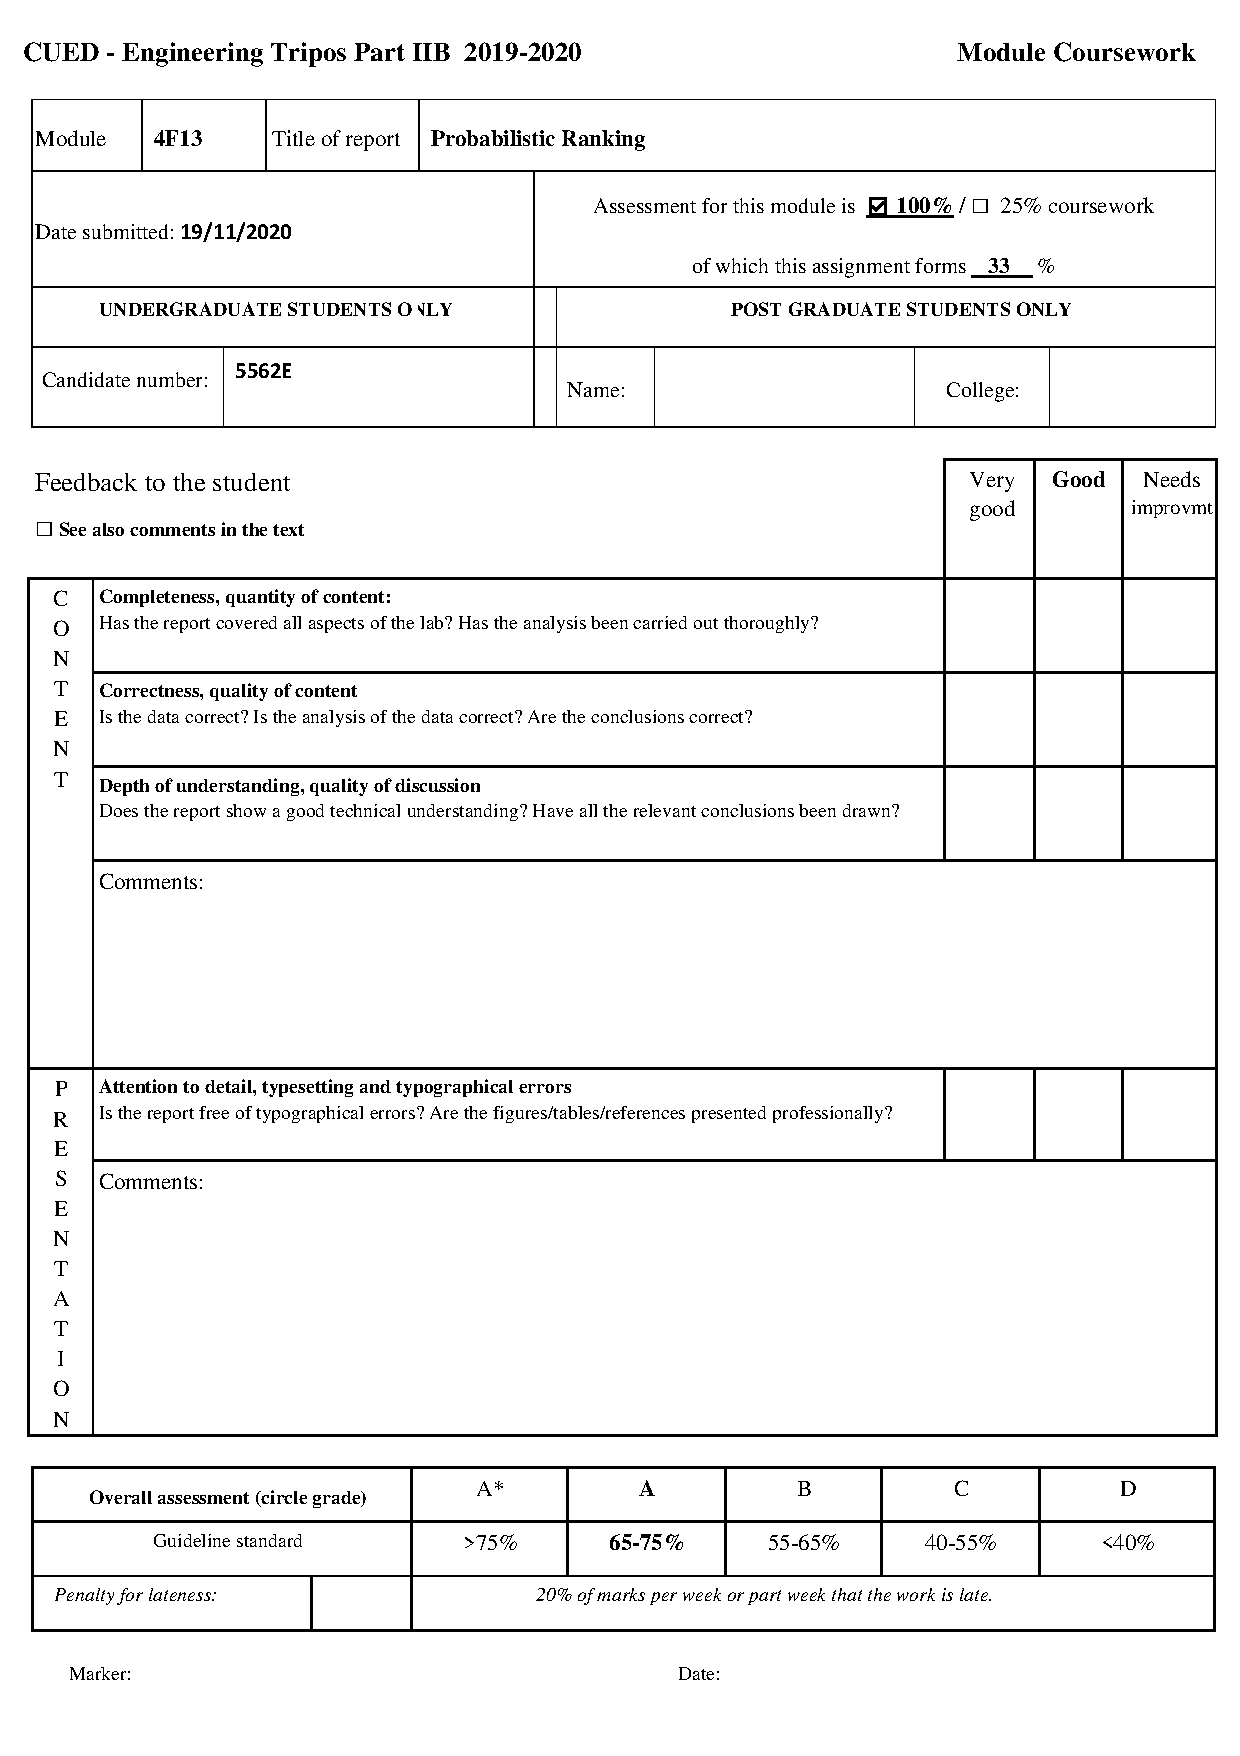
\includepdf[pages={1}]{coversheet-CW2.pdf}

\setcounter{page}{1}
\maketitle

\begin{abstract}
This report outlines the results of the second coursework for 4F13. We seek to rank professional tennis players based on game outcomes. We use the True-Skill model and apply Gibbs sampling as well as Expectation Propagation to the dataset. Both methods produce results that are in broad agreement. Nevertheless, EP is more computationally efficient.

The Gibbs sampler must be afforded a burn-in period to ensure the Markov chain is stationary and then the samples are thinned to ensure approximate independence. EP does not suffer from these weaknesses though it only returns estimates for the parameters of each player and not cross-correlation terms. This means that player comparison may be slightly less accurate for EP.

A player's win ratio is a coarse predictor of skill though somewhat unsatisfactory as it fails to take into account the opposition in each match. This is the reason for the True-Skill model.
\end{abstract}

\tableofcontents

\pagebreak
\section{Questions}
\subsection{Gibbs Sampling}

Gibbs sampling is used to sample from a multi-variate distribution by sequentially sampling from univariate conditionals. In the True-Skill model, we can approximate the conditional distribution with a 1-D Gaussian of a certain mean and variance - which are functions of the other variables and game outcomes. A portion of the modified code to compute these samples is given in listing \ref{lst:gibbs}.

\begin{lstlisting}[frame=single, caption={Gibbs sampling additions}, label={lst:gibbs}, language={python}]
m = np.zeros((M, 1))
for p in range(M):
	# fill in m[p] prediction (natural param conditional)
	wins_array = np.array(G[:, 0] == p).astype(int)
	loss_array = np.array(G[:, 1] == p).astype(int)
	m[p] = np.dot(t[:,0], (wins_array - loss_array))
\end{lstlisting}

We plot the sampled player skills for a few players (figure \ref{fig:skill-samples-long}). These data do appear noisy (in some sense random) but it is hard to tell how soon the Gibbs sampler transitions into a stable probability density region.

\begin{figure}[!h]
	\centering
	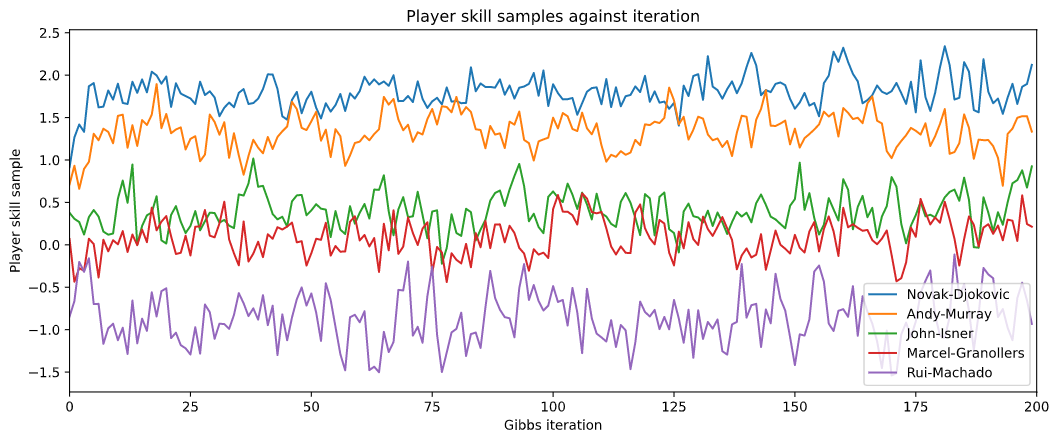
\includegraphics[width=0.8\linewidth]{skill-samples-long.png}
	\caption{Gibbs skill samples for various players}
	\label{fig:skill-samples-long}
\end{figure}

To investigate the burn-in time, we plot the population mean and standard deviation at each Gibbs iteration - figure \ref{fig:burn-in}. The population mean gives us little information but we see that the standard deviation converges to a steady value fairly quickly (only after 10 iterations). We set the burn-in time to $b=10$ and discard all preceding samples. 

\begin{figure}[!h]
	\centering
	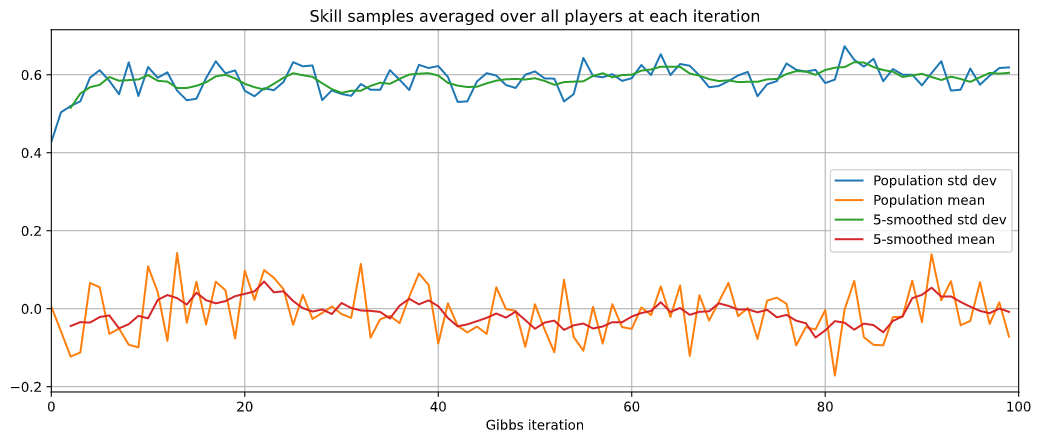
\includegraphics[width=0.8\linewidth]{burn-in.png}
	\caption{Gibbs skill samples averaged over all players at each iteration}
	\label{fig:burn-in}
\end{figure}

However, there is an additional wrinkle, the plot in figure \ref{fig:skill-samples-long} is smoother than it should be; neighbouring samples are not independent. To test this hypothesis, we plot the auto-correlation of each player's skill samples (figure \ref{fig:auto-cor}). For samples to be approximately independent, their correlation should be close to 0. We get good enough for an offset of $t=5$ - excepting one player: Djokovic.

\begin{figure}[!h]
	\centering
	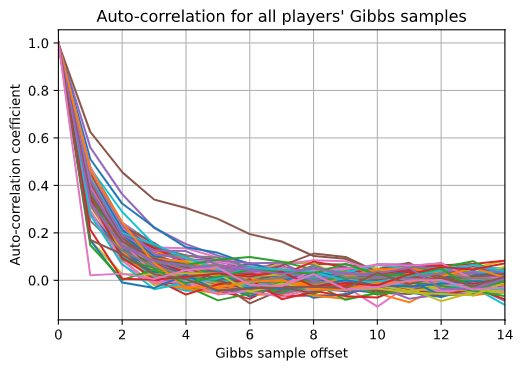
\includegraphics[width=\figwidth]{auto-cor.png}
	\caption{Auto-correlation for Gibbs sampler for all players}
	\label{fig:auto-cor}
\end{figure}

In summary, to run our Gibbs sampler reliably, we only use samples after a burn-in period of $b=10$ iterations. Even then, we thin the samples such that we only keep every $t$'th ($t=5$) sample to ensure that they are approximately independent. We use these values $b=10$ and $t=5$ for the rest of the report.

\subsection{EP - Message Passing}

Nevertheless, Gibbs sampling is rather computationally intensive. An alternative is message-passing through the Expectation Propagation (EP algorithm). This treats each player as a vertex on a graph, connected by directed edges representing game outcomes. We can use message passing (a form of Belief Propagation) to iteratively improve on our guess for each player's marginal skill. We approximate the marginal skill by a Gaussian with two parameters: mean and precision (inverse variance). These parameters have the advantage of combining simply to form the messages.

In Gibbs sampling, we run a Markov chain and aim to converge to a stationary probability distribution. This target distribution is the joint player skill distribution. However, in EP we do not converge to a distribution but rather a stable graph object; further iterations do not alter the parameters of each vertex: mean and precision.

In the previous section, we saw the Gibbs sampler only takes $b=10$ samples to converge to a stationary distribution. For the EP algorithm, we can plot the player parameters against iteration number for a few players to gauge convergence (figure \ref{fig:ep-evolution}).

\begin{figure}[!h]
	\begin{subfigure}{0.5\linewidth}
		\centering
		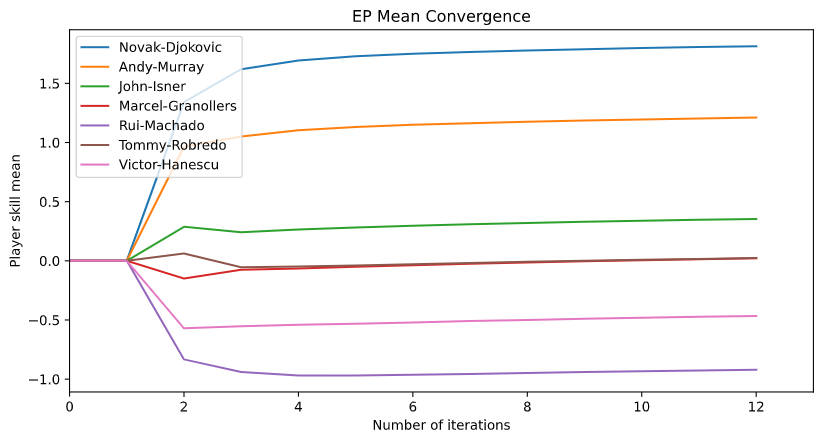
\includegraphics[width=\linewidth]{ep-mean.png}
		\caption{EP player skill mean evolution}
		\label{fig:ep-mean}
	\end{subfigure}
	\begin{subfigure}{0.5\linewidth}
		\centering
		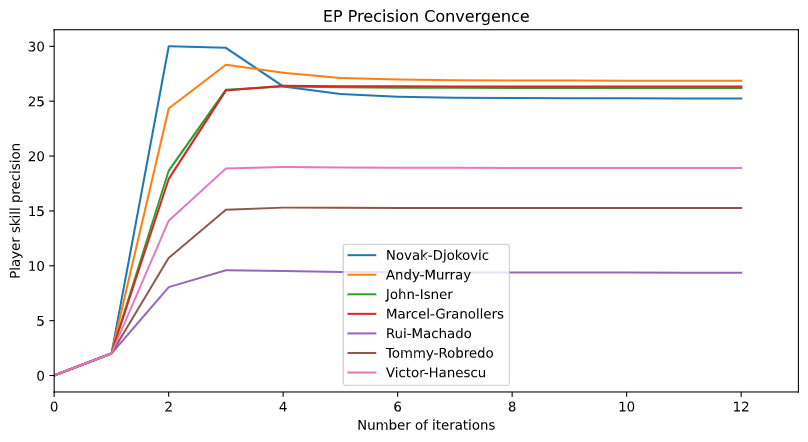
\includegraphics[width=\linewidth]{ep-precision.png}
		\caption{EP player skill precision evolution}
		\label{fig:ep-precision}
	\end{subfigure}
	\caption{EP player skill parameter evolution against iteration}
	\label{fig:ep-evolution}
\end{figure}

From the plots we can tell that we converge quickly for this set of players. Setting the number of iterations to $T=5$ seems reasonable to get a good estimate of the rankings as the mean and precision do not change much after this point. This value of $T=5$ will be used throughout the rest of the report.

\clearpage
\subsection{EP - Player Comparison}

Suppose that a player $i$ goes up against $j$. In the True-Skill model, we denote their skill by $w_i \sim \Ncal(m_i, \sigma_i^2)$ and $w_j \sim \Ncal(m_j, \sigma_j^2)$ respectively. The mean and variance parameters are estimated through message passing (the variance is just the inverse of the precision). 

The performance difference $s_{ij} = w_i - w_j$ is corrupted by Gaussian noise of unit variance $t_{ij} = s_{ij} + n$ to account for performance inconsistency ($n \sim \Ncal(0, 1)$). The match result is then given by the sign of $t_{ij}$ such that $t_{ij} > 0 \Rightarrow i \text{ wins}$ and j wins otherwise.

Having run message-passing, we wish to compute the probability that $i$ is more skilful than $j$: $P(s_{ij} > 0)$. This is different from the probability that $i$ beats $j$ in a head-to-head: $P(t_{ij} > 0)$. These probabilities are easy to compute by assuming that $w_i \indep w_j \indep n \indep w_i$, so means and variances combine additively:
%
\begin{align}
		s_{ij} = w_i - w_j &\sim \Ncal(m_i - m_j, \sigma_i^2 + \sigma_j^2)
		\label{eqn:s-ij} \\	
		t_{ij} = s_{ij} + n &\sim \Ncal(m_i - m_j, \sigma_i^2 + \sigma_j^2 + 1)
		\label{eqn:t-ij}
\end{align}

For any Gaussian r.v. $X \sim \Ncal(\mu, \sigma^2)$, $P(X > 0) = \Phi(\mu / \sigma)$ - where $\Phi(\cdot)$ is the standard Gaussian c.d.f. Applying this result to equations \ref{eqn:s-ij} and \ref{eqn:t-ij} for the top four ranked players, we obtain table \ref{tab:top-4}.

\begin{table}[!h]
	\subfloat[Prob. row player is more skilful]{
		\begin{tabular}{c | c c c c}
			$P(s_{ij} > 0)$ & \textbf{Djokovic} & \textbf{Federer} & \textbf{Nadal} & \textbf{Murray} \\ \hline
			\textbf{Djokovic}      & -                 & 0.91             & 0.94           & 0.99            \\
			\textbf{Federer}       & 0.09              & -                & 0.58           & 0.81            \\
			\textbf{Nadal}         & 0.06              & 0.42             & -              & 0.76            \\
			\textbf{Murray}        & 0.01              & 0.19             & 0.24           & -              
		\end{tabular}
		\label{tab:top-4-skills}
	}
	\subfloat[Prob. row player wins a head-to-head]{
		\begin{tabular}{c | c c c c}
			$P(t_{ij} > 0)$ & \textbf{Djokovic} & \textbf{Federer} & \textbf{Nadal} & \textbf{Murray} \\ \hline
			\textbf{Djokovic}      & -                 & 0.64             & 0.66           & 0.72            \\
			\textbf{Federer}       & 0.36              & -                & 0.52           & 0.59            \\
			\textbf{Nadal}         & 0.34              & 0.48             & -              & 0.57            \\
			\textbf{Murray}        & 0.28              & 0.41             & 0.43           & -              
		\end{tabular}
		\label{tab:top-4-wins}
	}
	\caption{Top four players comparison based on EP (5 iterations)}
	\label{tab:top-4}
\end{table}

We are more confident in who is better than in who will win: $|P(s_{ij} > 0) - 0.5| > |P(t_{ij}) - 0.5| \quad \forall i,j$. This makes sense mathematically as the variance $\sigma_t^2 > \sigma_s^2$. It also makes sense intuitively because an individual match is subject to performance variation. I would bet my house that Djokovic is a better tennis player than Andy Murray, but I'm not betting that much on Djokovic winning his match against him tomorrow.

\clearpage
\subsection{Gibbs - Player Comparison}

However, we can also compare players through Gibbs sampling. Restricting ourselves to just Djokovic and Nadal, we compare them in three ways:

\begin{enumerate}
	\item Approximate marginals by Gaussian
	\item Approximate joint by bivariate Gaussian
	\item Empirical comparison of joint samples
\end{enumerate}

The first method is shown in figure \ref{fig:djok-nadal-marginal}. We estimate the parameters of each Gaussian by taking the mean and variance of each player's Gibbs samples (after accounting for burn-in and thinning). Indeed a Gaussian does seem to be a good fit for the data. We see that Djokovic has higher mean and lower variance.

\begin{figure}[!h]
	\centering
	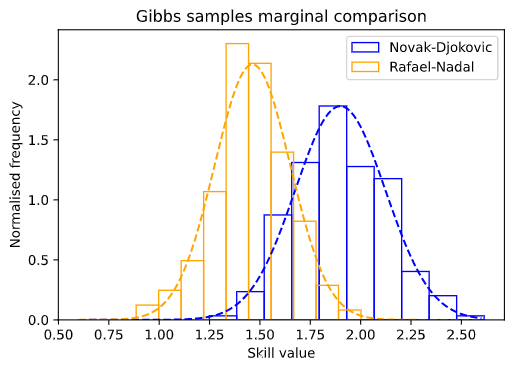
\includegraphics[width=\figwidth]{djokovic-nadal-marginal.png}
	\caption{Gibbs samples marginal comparison - Djokovic v Nadal}
	\label{fig:djok-nadal-marginal}
\end{figure}

Instead we can fit a bivariate Gaussian to the pair-wise samples $\{(w_i^{(n)}, w_j^{(n)})\}_{n=1}^{N}$ (figure \ref{fig:djok-nadal-joint}). We approximate the parameters as before but now noting that we have an additional covariance term $\sigma_{ij}^2$ off the diagonal of the $2 \times 2$ variance matrix. This covariance term is non-zero (in fact positive) meaning that the principal axes of the Gaussian are slightly skewed.

\begin{figure}[!h]
	\centering
	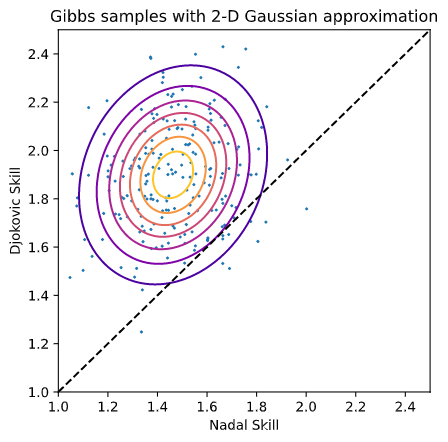
\includegraphics[width=\figwidth]{djokovic-nadal-joint.png}
	\caption{Gibbs samples joint comparison - Djokovic v Nadal}
	\label{fig:djok-nadal-joint}
\end{figure}

The last method involves simply plotting the difference of the two skill samples (figure \ref{fig:djok-nadal-diff}). Any bars coloured red have Nadal higher skill than Djokovic.

\begin{figure}[!h]
	\centering
	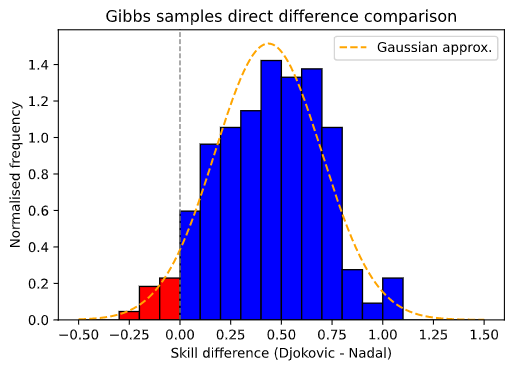
\includegraphics[width=\figwidth]{djokovic-nadal-diff.png}
	\caption{Gibbs samples direct difference comparison - Djokovic v Nadal}
	\label{fig:djok-nadal-diff}
\end{figure}

Each of these methods give a different way of estimating the probability player $i$ is more skilful than $j$: $P(s_{ij} > 0)$. They are listed below:

\begin{enumerate}
	\item Independent Gaussians - $\Phi((m_i - m_j)/(\sigma_i^2 + \sigma_j^2))$
	\item Correlated Gaussians - $\Phi((m_i - m_j)/(\sigma_i^2 - 2\sigma_{ij}^2 + \sigma_j^2))$
	\item Empirical comparison - $N^{-1} \sum_{n=1}^{N} \mathbbm{1} (w_i^{(n)} > w_j^{(n)})$
\end{enumerate}

Figure \ref{fig:djok-nadal-joint} shows that the samples are not independent so method 2 is preferred over 1. In addition, as the probabilities can be very small, the empirical estimate (though unbiased) will need a very high number of samples $N$ to be accurate (the red area in figure \ref{fig:djok-nadal-diff} is very small). Therefore we prefer method 2 for comparing player skills. Doing this for the top four players yields table \ref{tab:top-4-gibbs}.

\begin{table}[!h]
	\centering
	\begin{tabular}{c | c c c c}
		$P(s_{ij} > 0)$ & \textbf{Djokovic} & \textbf{Federer} & \textbf{Nadal} & \textbf{Murray} \\ \hline
		\textbf{Djokovic}      & -                 & 0.92             & 0.95           & 0.98            \\
		\textbf{Federer}       & 0.08              & -                & 0.63           & 0.81            \\
		\textbf{Nadal}         & 0.05              & 0.37             & -              & 0.75            \\
		\textbf{Murray}        & 0.02              & 0.19             & 0.25           & -              
	\end{tabular}
	\caption{Player skills head-to-head - $P(s_{ij} > 0) = \Phi((m_i - m_j)/(\sigma_i^2 - 2\sigma_{ij}^2 + \sigma_j^2))$}
	\label{tab:top-4-gibbs}
\end{table}

Table \ref{tab:top-4-gibbs} agrees with \ref{tab:top-4-skills} very well. If anything the predictions tend to be more confident for the joint Gaussian model as the covariance between each of the top four players' skills is positive. Therefore, this decreases the variance of the difference, leading to more confident predictions.

\clearpage
\subsection{Method Comparison: Win ratio, Gibbs and EP}

We go about ranking players using different methods: win ratio; Gibbs sampling for the True-Skill model; and EP estimates for True-Skill.

The win ratio model assumes that each player has a fixed probability of winning their match irrespective of their opponent. If a player has played $n$ matches and won $k$ of them, we know their win ratio is distributed as $p \sim \Ncal(k/n, k(n-k)/n^2)$; this applies standard results for combining $n$ independent Bernoulli r.v.'s.

With Gibbs sampling, we sample the player skill from conditionals such that we mimic sampling from the joint. After burn-in and thinning, we have a set of independent samples for the skill of each player and we can calculate the mean and variance of this set empirically.

For Expectation Propagation, we run the Message Passing algorithm for 5 iterations to achieve convergence. This returns the expected means and precisions (inverse variance) for the skill of each player.

\begin{figure}[!h]
	\centering
	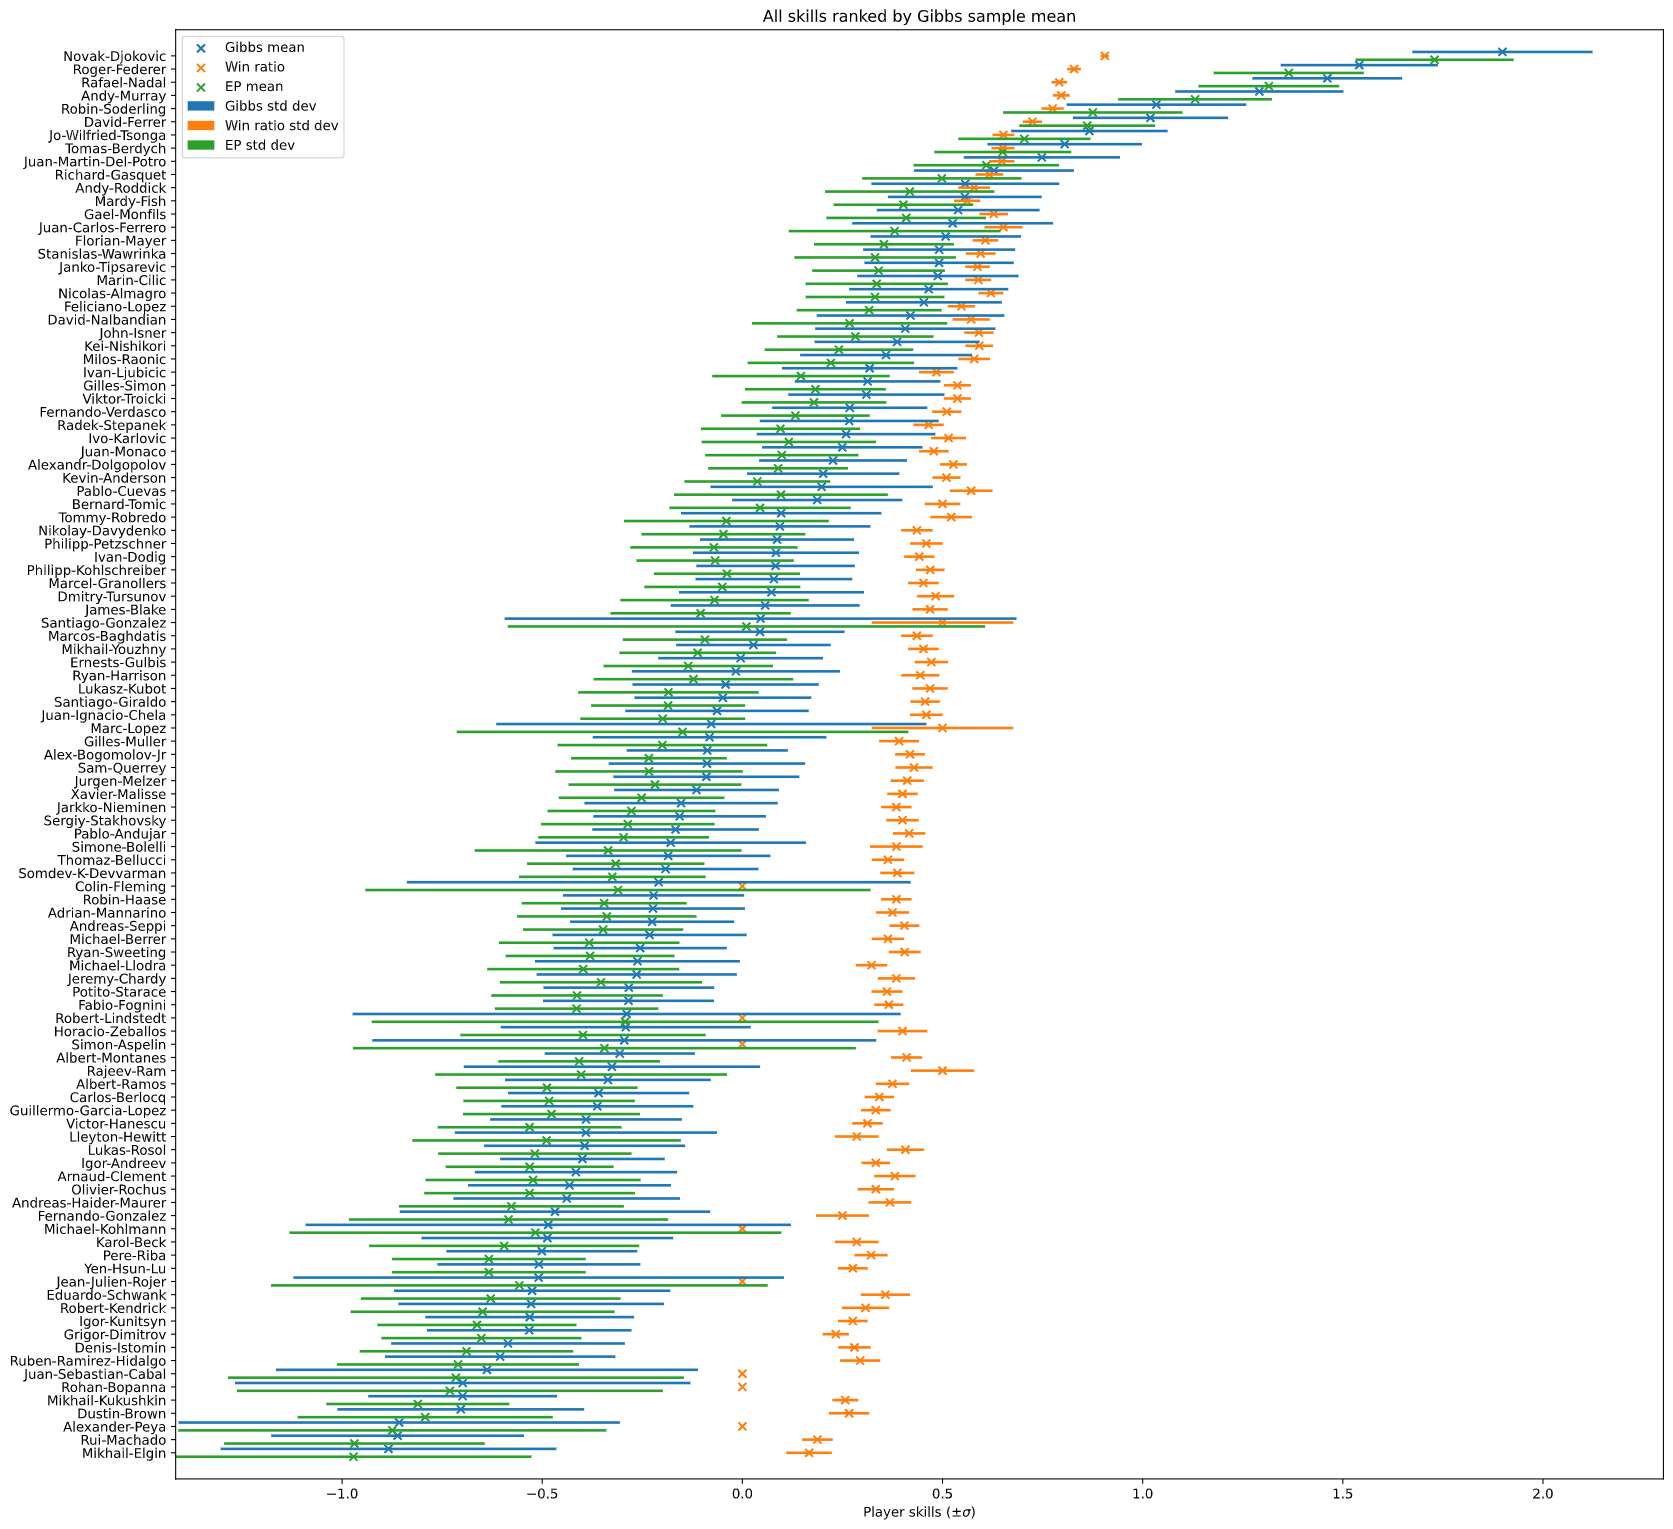
\includegraphics[width=\linewidth]{combined-ranking.png}
	\caption{Player skills ranked by Gibbs sample mean}
	\label{fig:combined-ranking}
\end{figure}

We plot all three methods on figure \ref{fig:combined-ranking} - rank ordering by Gibbs sample mean. Right away we see excellent agreement between the Gibbs and EP datasets. They seem to differ only by a constant and a small amount of noise. The constant offset does not matter when comparing players but it is determined by the prior $p(w) \sim \Ncal(0, 1)$. It is possible that the EP algorithm drifts away from this prior after initialisation. The noise we see (slight discrepancies in rank order) may be due to approximation errors from each approach. Nevertheless, the variances of both Gibbs and EP match closely.

As for the win ratio, its rank ordering does not agree especially well with the other two. This is to be expected as the win ratio does not factor in who the opposition is when determining a rank ordering. Nonetheless, the general trend of higher win ratios meaning higher skill is preserved. It is interesting to note that there are several players with a win ratio of 0 who are moderately high up on the Gibbs rankings (e.g. Colin Fleming). This means that they must have played very few games (losing all of them) and so their mean stays close to the prior mean of 0 albeit with high variance. If we increased the prior variance, we would see fewer players with no wins to their name appearing so high up in the rankings.

\textbf{Words}: XX

\end{document}
